% !TeX spellcheck = en_GB
%%%%%%%%%%%%%%%%%%%%%%%%%%%%%%%%%%%%%%%%%%%%%%%%%%%%%%%%%%%%%%%%%%%%%%%%%%%%%%%%
%\documentclass[handout]{beamer}\mode<handout>{\usetheme{default}}
%
%\documentclass[presentation]{beamer}\mode<presentation>{\usetheme{blackAMSBolognaFC}}
\documentclass[handout]{beamer}\mode<handout>{\usetheme{AMSBolognaFC}}
% \setbeamertemplate{bibliography item}{\insertbiblabel}
%%%%%%%%%%%%%%%%%%%%%%%%%%%%%%%%%%%%%%%%%%%%%%%%%%%%%%%%%%%%%%%%%%%%%%%%%%%%%%%%
\usepackage[english]{babel}
\usepackage[utf8]{inputenc}
\usepackage[labelformat=empty]{caption}
\usepackage{listings}
\usepackage{tabularx}
\usepackage{subcaption}
\usepackage[most]{tcolorbox}
%
\usepackage{talk-2024-aixia-rag}
%%%%%%%%%%%%%%%%%%%%%%%%%%%%%%%%%%%%%%%%%%%%%%%%%%%%%%%%%%%%%%%%%%%%%%%%%%%%%%%%
\title[RAG on LLMs for Medical Chatbot]{%
    % same title of the presented paper
    \small{
        \large{
            Applying Retrieval-Augmented Generation on Open LLMs
            \\
            for a Medical Chatbot Supporting Hypertensive Patients
        }
    }
}
%
% \subtitle{Extended Abstract}
%
% same authors order of the presented paper
\author[Aguzzi et al.]{
	Gianluca Aguzzi$^{*}$ % empth the presenting author
	\and 
	Matteo Magnini$^{*}$
	\and
	Giuseppe Pio Salcuni$^{*}$
	\\
	Stefano Ferretti$^{*}$
    \and
    \emph{Sara Montagna$^{\dagger}$}
}
%
\institute[UniBo, UniUrb]{
    $^{*}$Department of Computer Science and Engineering (DISI)
    \\
    \textsc{Alma Mater Studiorum} -- University of Bologna
    \\
    \texttt{
        \{gianluca.aguzzi, matteo.magnini, stefano.ferretti\}@unibo.it
    }
    \\
    \texttt{
        giuseppepio.salcuni@studio.unibo.it
    }
    \vspace{.3cm}
    \\
    $^{\dagger}$Department of Pure and Applied Sciences (DiSPeA)
    \\
    University of Urbino
    \\
    \texttt{\emph{sara.montagna}@uniurb.it}
}
%
\date[HC@AIxIA, 2024]{
    \small{
        \small{
            3rd AIxIA Workshop on Artificial Intelligence For Healthcare (HC@AIxIA)
            \\
            27-28 November 2024, Bolzano, Italy
        }
    }
}
%%%%%%%%%%%%%%%%%%%%%%%%%%%%%%%%%%%%%%%%%%%%%%%%%%%%%%%%%%%%%%%%%%%%%%%%%%%%%%%%
\AtBeginSection[]
{
%\\\\\\\\\\\\\\\\\\\\\
\begin{frame}<beamer>[c,noframenumbering]
\frametitle{Next in Line\ldots}
\tableofcontents[sectionstyle=show/shaded,subsectionstyle=hide]
\end{frame}
%\\\\\\\\\\\\\\\\\\\\\
}
\AtBeginSubsection[]
{
%\\\\\\\\\\\\\\\\\\\\\
\begin{frame}<beamer>[shrink,noframenumbering]
    \frametitle{Focus on\ldots}
	\mbox{~}
	\tableofcontents[currentsubsection,sectionstyle=shaded,subsectionstyle=show/shaded]
	\mbox{~}
\end{frame}
%\\\\\\\\\\\\\\\\\\\\\
}
%%%%%%%%%%%%%%%%%%%%%%%%%%%%%%%%%%%%%%%%%%%%%%%%%%%%%%%%%%%%%%%%%%%%%%%%%%%%%%%%
\begin{document}
%%%%%%%%%%%%%%%%%%%%%%%%%%%%%%%%%%%%%%%%%%%%%%%%%%%%%%%%%%%%%%%%%%%%%%%%%%%%%%%%

%\\\\\\\\\\\\\\\\\\\\\
\frame{\titlepage}
%\\\\\\\\\\\\\\\\\\\\\

%===============================================================================
\section{Motivation \& Context}
%===============================================================================

%\\\\\\\\\\\\\\\\\\\\\
\begin{frame}[c]{Context}
    
    Chronic Disease Management Challenges
    %
    \vfill
    %
    \begin{itemize}
        %
        \item Managing chronic diseases is \alert{costly} and \alert{time-intensive}
        \item Engagement of patient is crucial for success
        %
    \end{itemize}
    \vfill
    \centering
    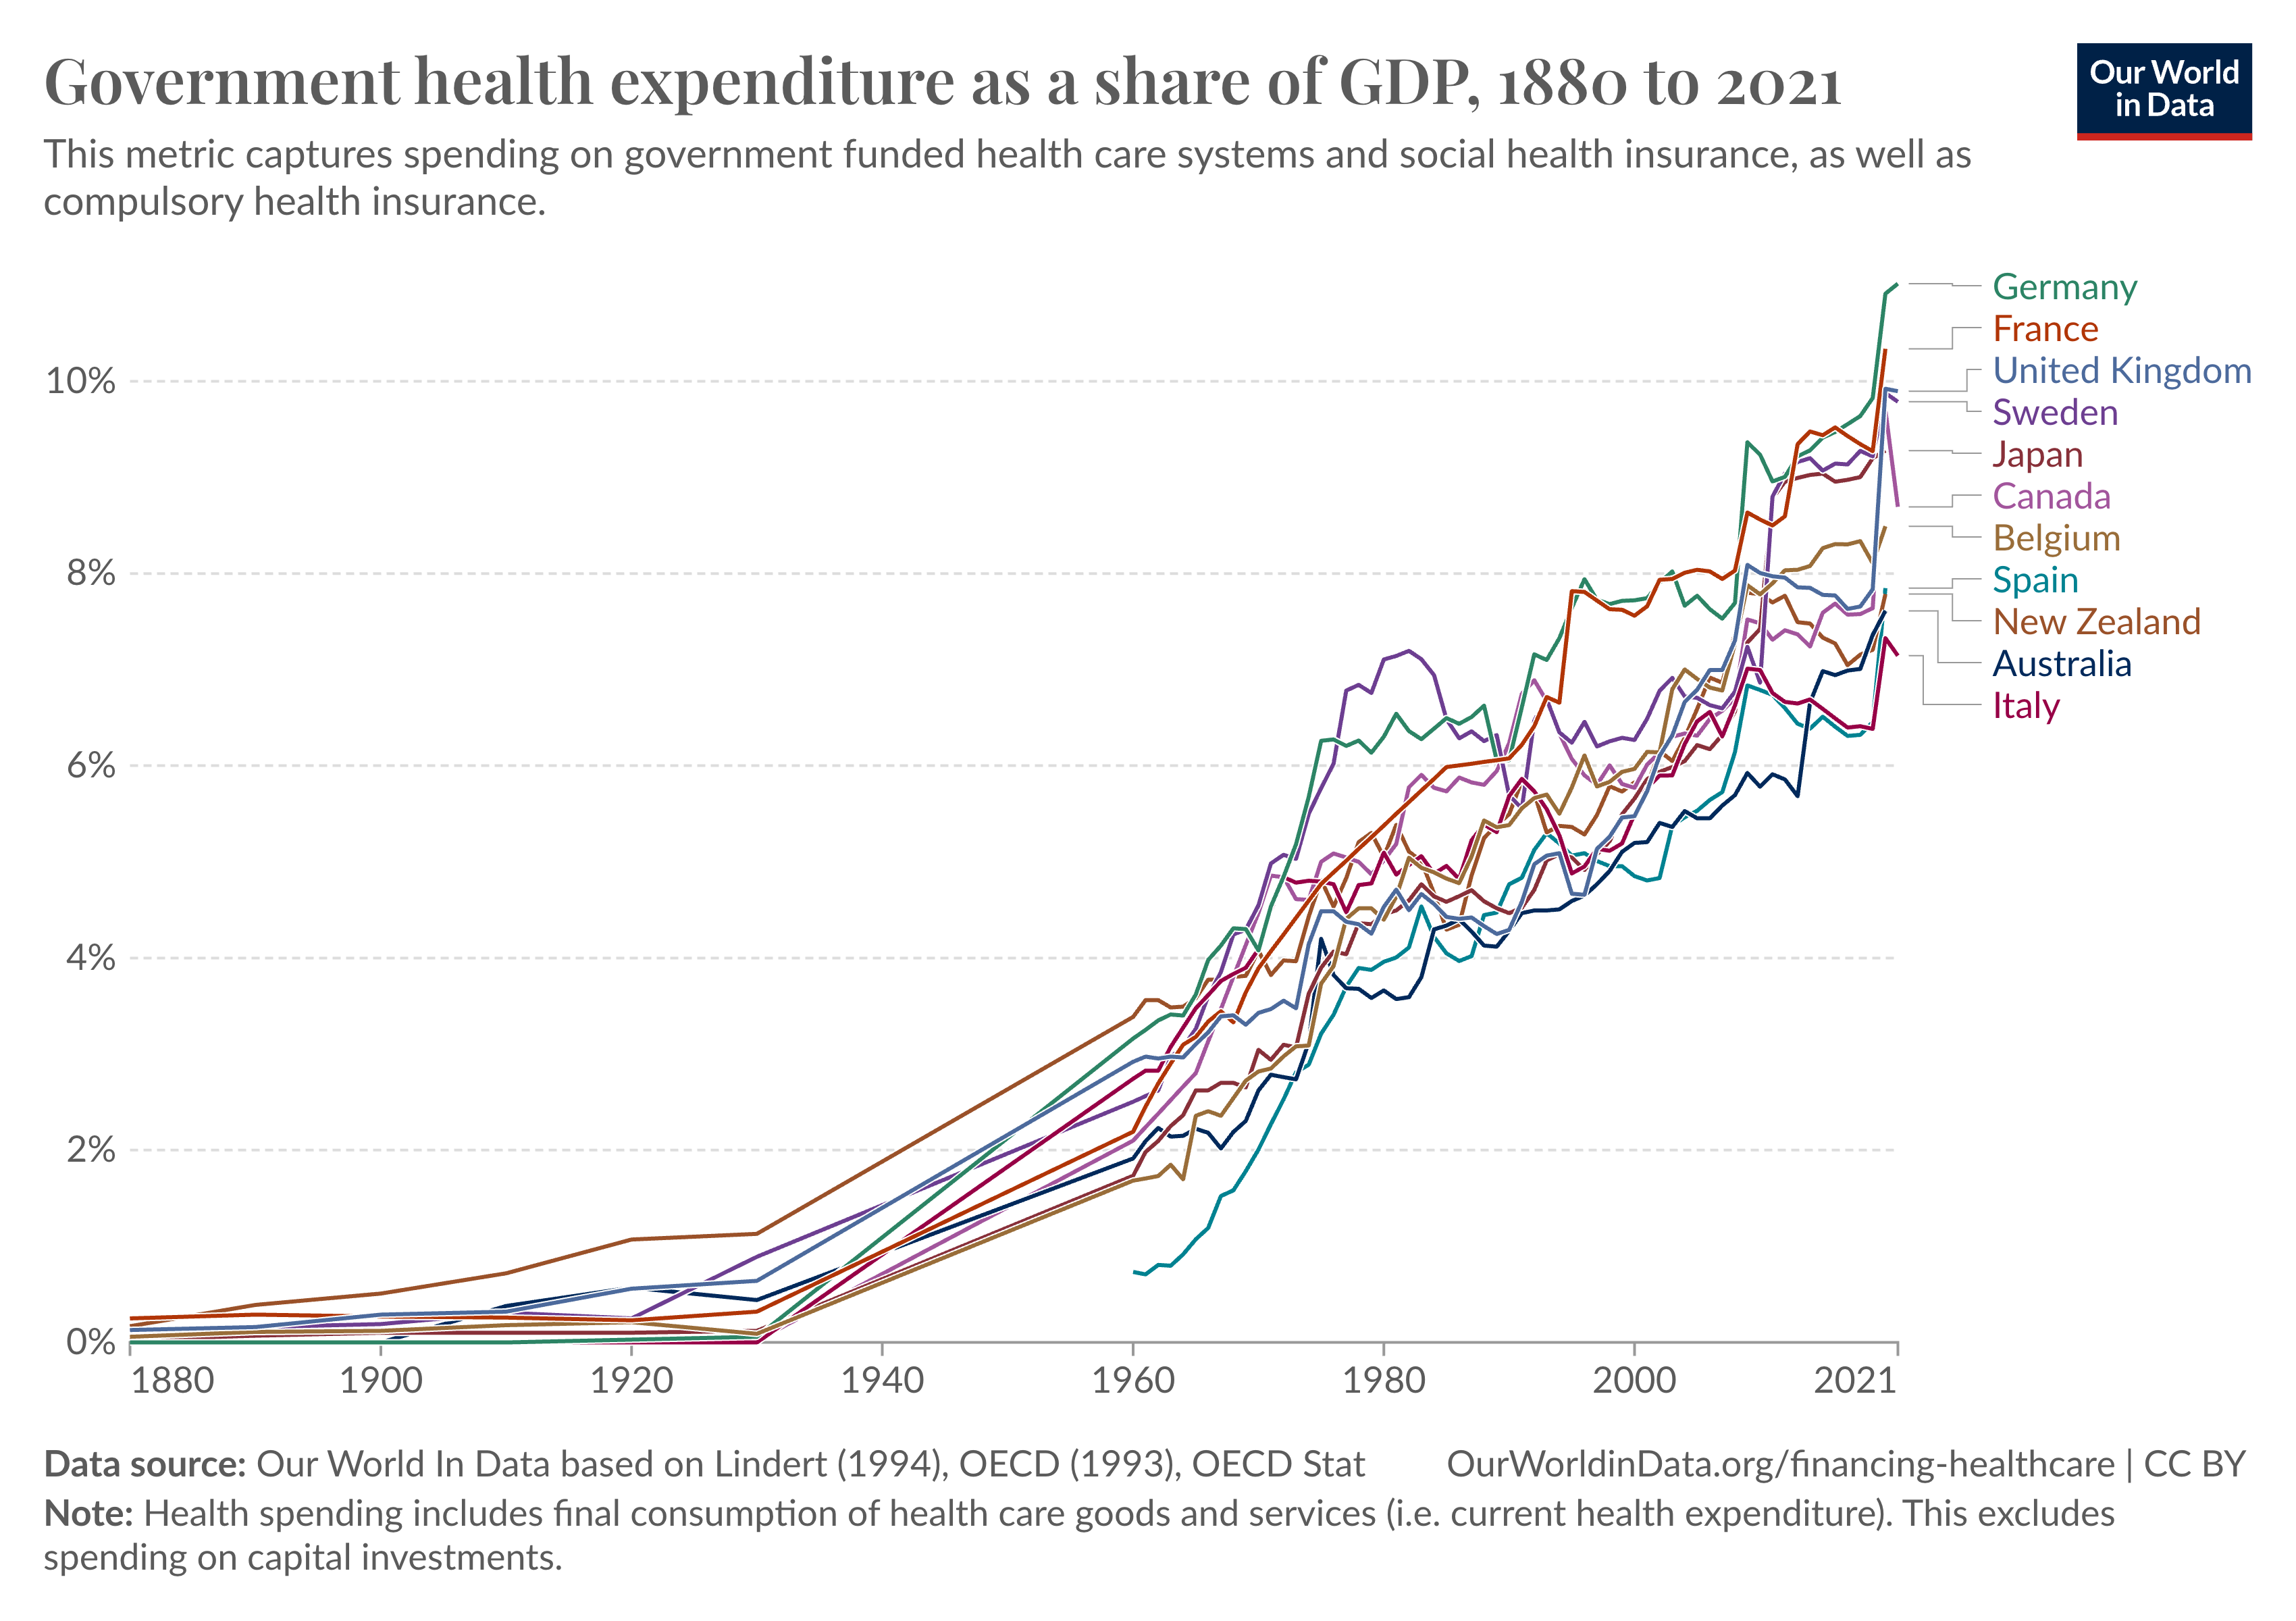
\includegraphics[width=.6\textwidth]{figures/public-health-expenditure-share-gdp}
    \vfill

\end{frame}
%\\\\\\\\\\\\\\\\\\\\\

%\\\\\\\\\\\\\\\\\\\\\
\begin{frame}[c]{Motivation}
    Why a Medical Chatbot for Hypertension?~\ccite{telmed2024}
    %
    \vspace{1em}
    %
    \begin{itemize}
        %
        \item Hypertension management requires ongoing support
        %
        \begin{itemize}
            \item \alert{monitoring}
            %
            \item \alert{guidance}
            %
        \end{itemize}
        %
        \item A personal digital assistant may reduce physicians workload and provide continuous \\ support to patients
        %
        \end{itemize}
        
 \vspace{-2.5em}
    \raggedleft
    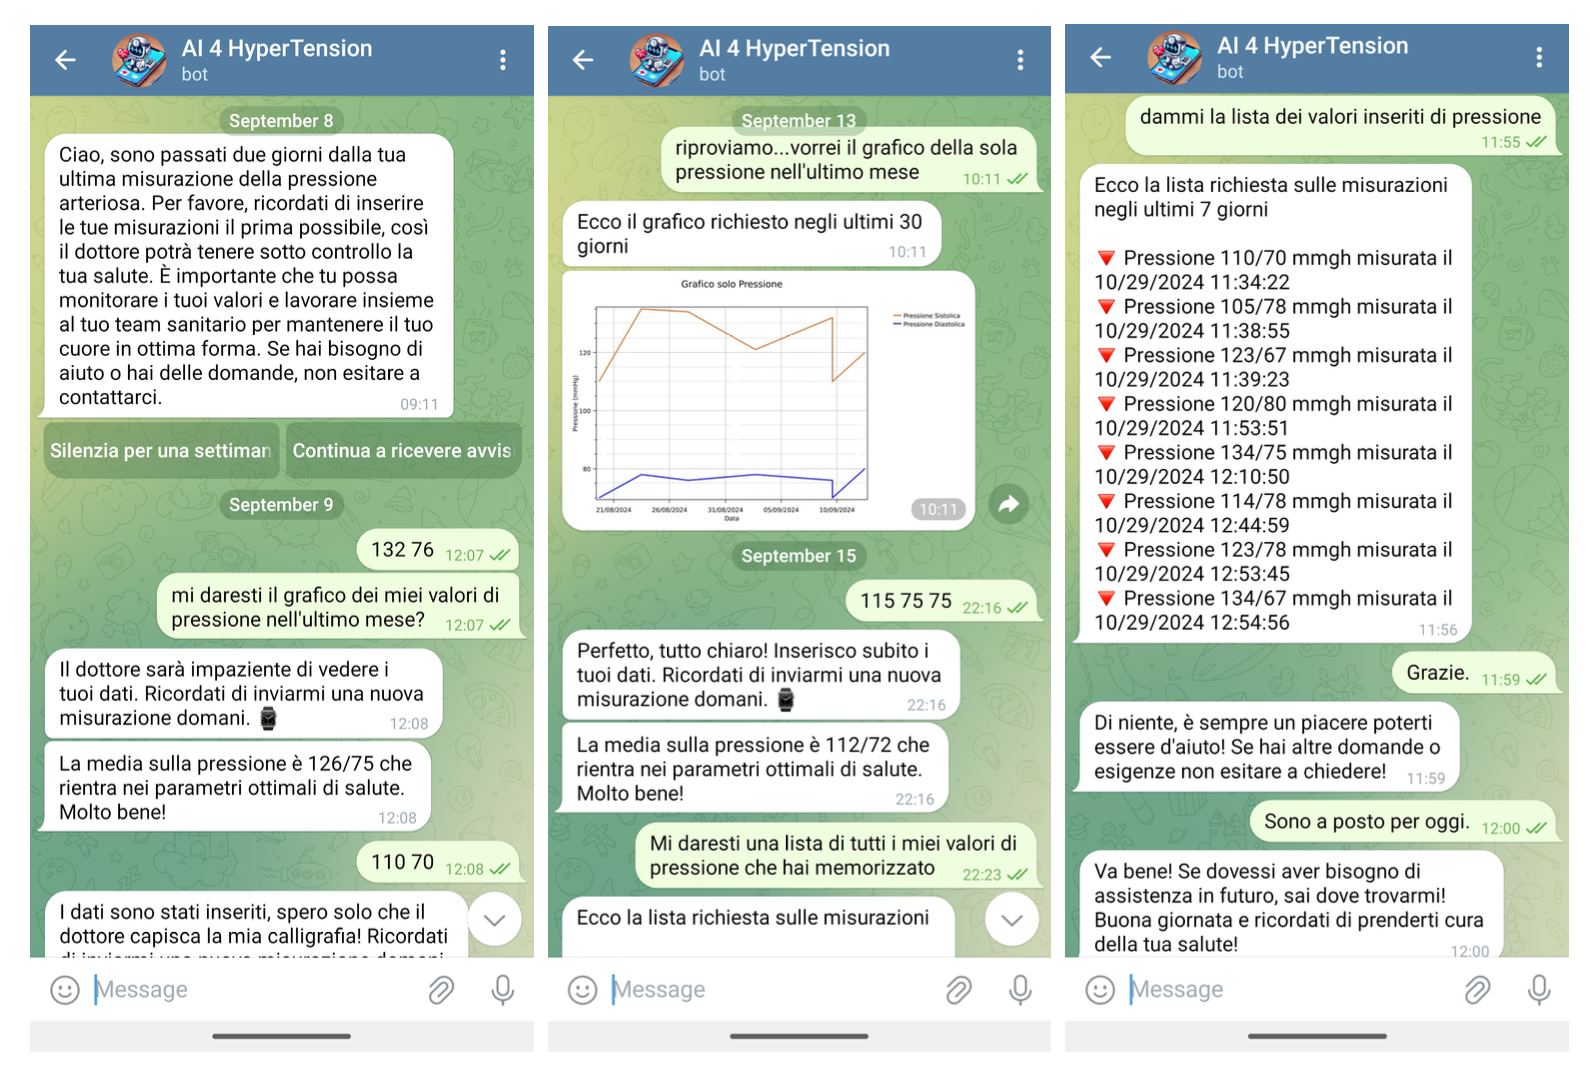
\includegraphics[width=.65\textwidth]{figures/chatbot}
    \vfill

\end{frame}
%\\\\\\\\\\\\\\\\\\\\\

%\\\\\\\\\\\\\\\\\\\\\
\begin{frame}{Contribution}

 \begin{block}{Requirements}
 	\begin{itemize}
 	%
        \item Need for high \alert{accuracy} and strong \alert{privacy} protection
        %
        \end{itemize}
\end{block}

    \begin{block}{Main contributions of our work}
        \begin{itemize}
            %
            \item Improved our chatbot for hypertensive patients using \alert{open LLMs}
            %
            \begin{itemize}
            \item they  overcome privacy concerns but need enhanced accuracy and domain-specific knowledge
        		$\rightarrow$ quest for diminishing \alert{hallucinations}!
       		
	\end{itemize}
            \item Incorporated \alert{Retrieval-Augmented Generation (RAG)}~\ccite{Lewis-NIPS20} for enhanced performance
            %
            \item \alert{Evaluated} several open-source LLMs with and without RAG
        \end{itemize}
    \end{block}
    \vspace{-0.5em}
    \begin{figure}
        \begin{minipage}{0.3\textwidth}
            \centering
            
\includegraphics[width=0.6\textwidth]{figures/telegram-bot}
            \caption{Try me!}
        \end{minipage}
        \hspace{2cm}
        \begin{minipage}{0.3\textwidth}
            \centering
            
\includegraphics[width=0.6\textwidth]{figures/github-repo}
            \caption{Check the code!}
        \end{minipage}
        \hfill
        \label{fig:telegram-bot}
    \end{figure}


\end{frame}
%\\\\\\\\\\\\\\\\\\\\\

%===============================================================================
\section{Theory, Experiments \& Results}
%===============================================================================

%\\\\\\\\\\\\\\\\\\\\\
\begin{frame}[allowframebreaks]
\frametitle{Theory}
    %
    \begin{block}{The RAG system}
        \vfill
        %
        \begin{itemize}
            %
            \item Key components
            %
            \begin{itemize}
                \item \alert{Retriever} $\rightarrow$ finds relevant information
                %
                \item \alert{Generator} $\rightarrow$ generates responses based on retrieved information
                %
            \end{itemize}
            %
        \end{itemize}
    \end{block}
    \vfill
    \centering
    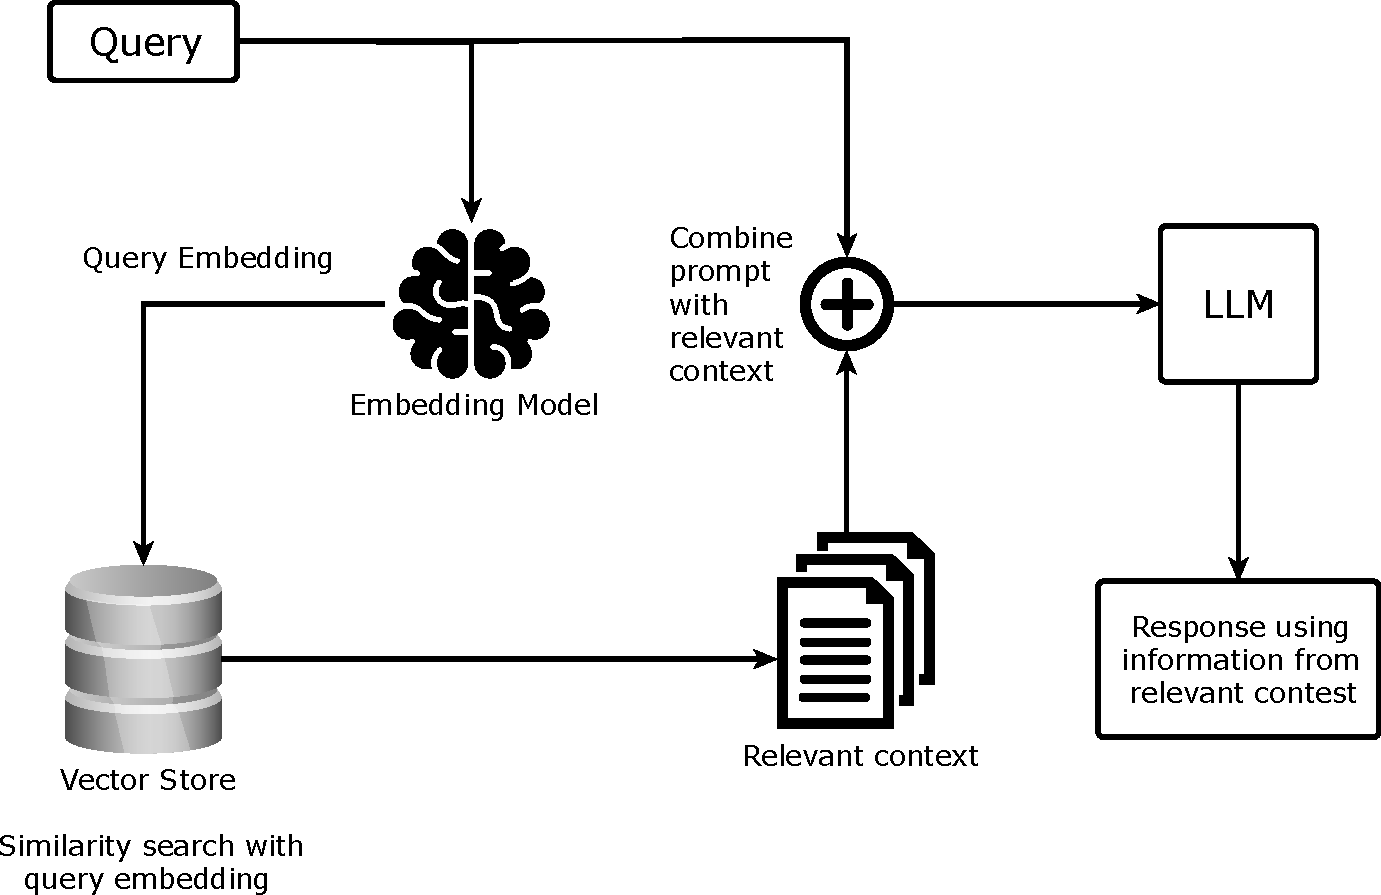
\includegraphics[width=.6\textwidth]{figures/rag-architecture}
    \vfill

    \framebreak

    \begin{block}{The RAG system}
        \begin{itemize}
            \item Data source $\rightarrow$ a collection of documents stored in a vector space
            \begin{itemize}
                \item[$\rightarrow$] in our case a collection of questions and answers verified by real doctors
            \end{itemize}
            %
            \item Different retrieval strategies
            %
            \begin{itemize}
                \item Base $\rightarrow$ vector similarity with the query
                %
                \item Ensemble $\rightarrow$ multiple retrievers
                %
                \item MultiQuery $\rightarrow$ multiple queries
            \end{itemize}
        \end{itemize}
    \end{block}
    %
    \begin{block}{Why RAG and not finetuning?}
        \begin{itemize}
            \item Multiple users, need to \alert{adapt} to different contexts
            %
            \item Fine-tuning LLMs is expensive and time-consuming
            %
            \item Avoid model \alert{drift}, \alert{hallucinations}, and other issues
        \end{itemize}
    \end{block}
\end{frame}
%\\\\\\\\\\\\\\\\\\\\\

%\\\\\\\\\\\\\\\\\\\\\
\begin{frame}{Experiments}

    \begin{block}{Experimental setup}
        \begin{description}[left=0pt]
            \item[Dataset]  \alert{1,473} question-answer pairs extracted from medical consultations
            \begin{itemize}
                \item[$\rightarrow$] questions cover a wide range of topics ---\alert{symptoms}, \alert{causes}, \alert{treatments}, and \alert{lifestyle recommendations}
            \end{itemize}
            %
            \item[Models]  both general-purpose models and medical-domain-specific models
            %
            \item[Metrics] We used three metrics to evaluate the performance of the models:
            \begin{itemize}
                \item[$\rightarrow$] \textbf{Answer relevancy}: assess the \alert{relevance} of the answer to the question
                \item[$\rightarrow$] \textbf{Answer correctness}: evaluate the \alert{correctness} of the answer
                \item[$\rightarrow$] \textbf{Faithfulness}: measure the \alert{alignment} between the answer and the retrieved information
            \end{itemize}
            %
        \end{description}
    \end{block}

\end{frame}

%\\\\\\\\\\\\\\\\\\\\\
\begin{frame}{Models}
    \tiny{
        \footnotesize{
            \begin{table}[htbp]
                \centering
                %\caption{Evaluated LLMs for our study.}
                \label{tab:evaluated-llms}
                \begin{tabular}{|l|p{0.6\textwidth}|}
                    \hline
                    \textbf{Model} & \textbf{Description} \\
                    \hline
                    Llama3.1 & A general-purpose LLM based on the Llama3 architecture with 8B parameters, trained on a diverse range of text data~\ccite{llama3}. \\
                    \hline
                    Llama3.1-Medical & A medical-domain-specific version of Llama3.1, fine-tuned to enhance its performance in healthcare. \\
                    \hline
                    Qwen2 & A 7B parameters general-purpose LLM, trained on 29 languages to improve cross-lingual performance~\ccite{qwen2}. \\
                    \hline
                    Qwen2-Medical & A medical-domain-specific version of Qwen2, fine-tuned to improve its performance in healthcare tasks. \\
                    \hline
                    Mistral-Nemo & A 12B parameter model with a large context window (128K tokens) developed by Nvidia. \\
                    \hline
                    Phi3 & A small LLM with 3B parameters, trained by Microsoft on filtered high-quality data~\ccite{abdin2024phi3technicalreporthighly}. \\
                    \hline
                    Gemma2 & A 9B parameter model based on Deepmind Gemini developed by Google~\ccite{gemmateam2024gemma2improvingopen}. \\
                    \hline
                \end{tabular}
            \end{table}
        }
    }
    \vfill

\end{frame}
%\\\\\\\\\\\\\\\\\\\\\

%\\\\\\\\\\\\\\\\\\\\\
\begin{frame}[allowframebreaks]
    \frametitle{Results}

    \begin{block}{RAG vs. No-RAG}
        \begin{itemize}
            \item RAG models outperformed No-RAG models in terms of \alert{correctness} (\alert{up to 20\%} ) and \alert{relevancy} (\alert{up to 40\%})
            %
            \item This strongly suggests that integrating external knowledge sources via RAG \alert{significantly improves} the quality of generated responses
            
        \end{itemize}
    \end{block}
     $\rightarrow$ the RAG approach demonstrates to be effective in domain-specific tasks, such as the medical one but\ldots
     
    \begin{block}{RAG strategies}
        \begin{itemize}
          %
            \item The choice of retrieval strategy significantly influenced the performance of the RAG systems
            %
         \end{itemize}
    \end{block}


    
    \framebreak

    \vfill
    \centering
    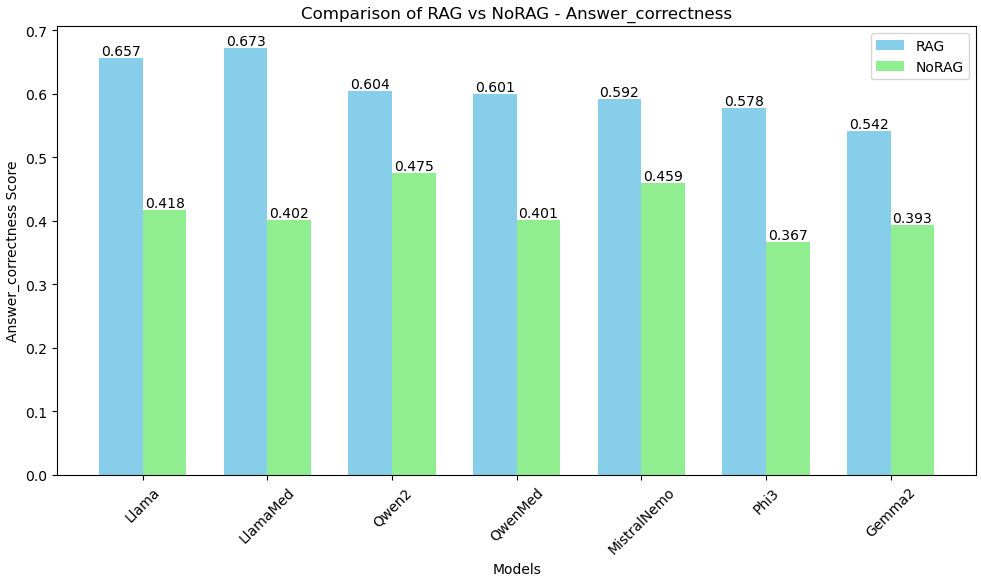
\includegraphics[width=\textwidth]{figures/RAGvsNoRAG_correctness}

    \framebreak

    \vfill
    \centering
    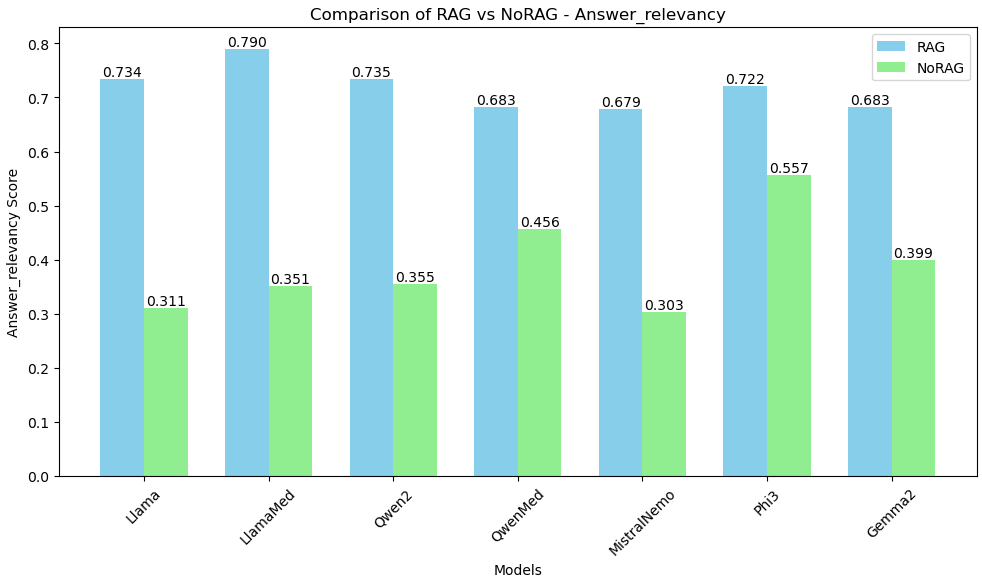
\includegraphics[width=\textwidth]{figures/RAGvsNoRAG_relevancy}

    \framebreak

    \vfill
    \centering
    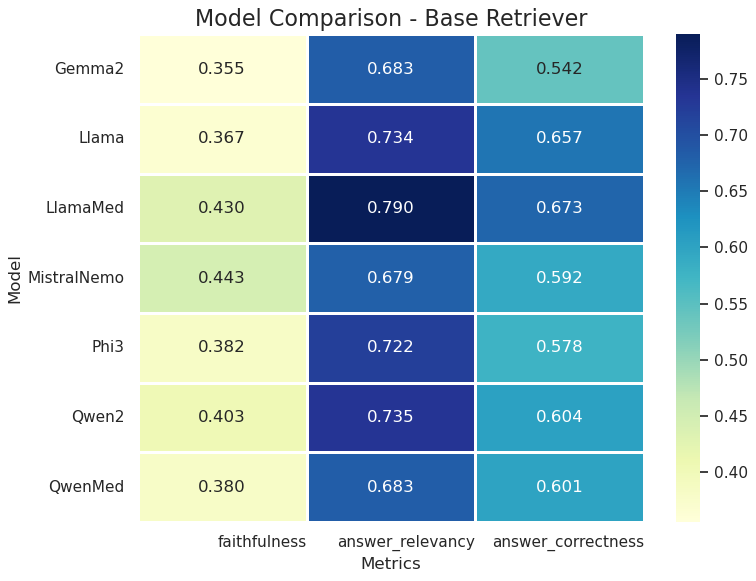
\includegraphics[height=0.8\textheight]{figures/baseretreiver}

    \framebreak

    \vfill
    \centering
    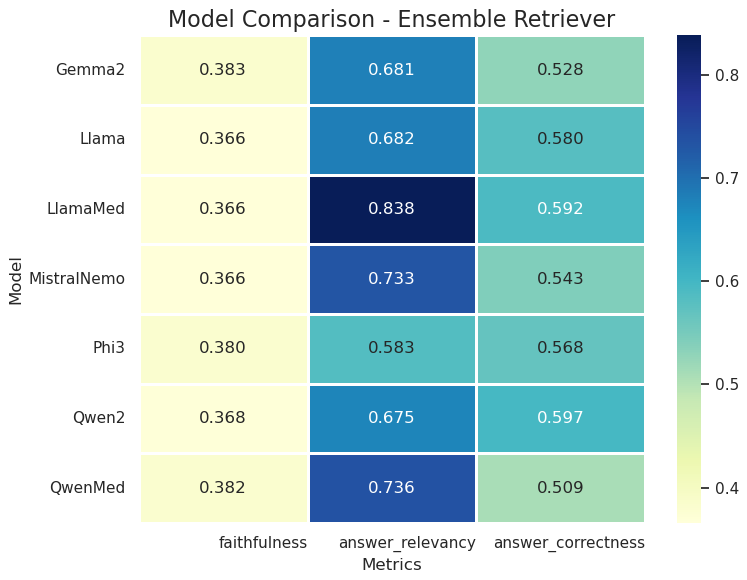
\includegraphics[height=0.8\textheight]{figures/ensembleretriever}

    \framebreak

    \vfill
    \centering
    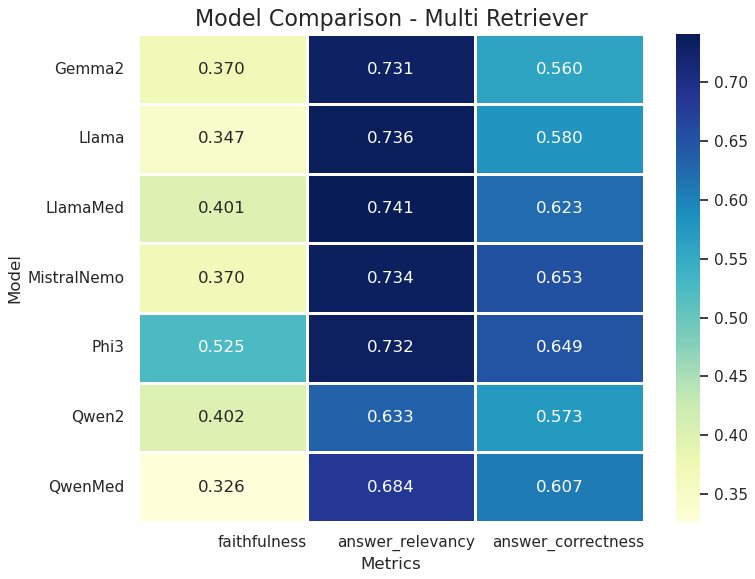
\includegraphics[height=0.8\textheight]{figures/multiretriever}

\end{frame}

%===============================================================================

\section{Conclusions \& future works}

%\\\\\\\\\\\\\\\\\\\\\
\begin{frame}%[allowframebreaks]
\frametitle{Conclusions \& future works}

\begin{block}{Summing up}
    \begin{itemize}
        \item We have shown that RAG can \alert{significantly improve} the performance of open LLMs in a medical chatbot context
        %
        \item RAG models \alert{outperform} No-RAG models in w.r.t. correctness and relevancy
        %
        \item The choice of \alert{retrieval strategy influences the performance}
    \end{itemize}
\end{block}

\begin{exampleblock}{Future works}
    %
    Future research should focus on two key areas:
    %
    \begin{itemize}
        \item Incorporating human evaluation by medical professionals to assess the clinical accuracy and appropriateness of the chatbot’s responses
        %
        \item Developing and integrating metrics specifically designed to evaluate the empathy and emotional intelligence of the chatbot’s communication
        %
    \end{itemize}
\end{exampleblock}

(may be split into 2 slides)

\end{frame}
%\\\\\\\\\\\\\\\\\\\\\

%===============================================================================
\section*{}
%===============================================================================
\frame{\titlepage}

%===============================================================================
\section*{\bibname}
%===============================================================================

\setbeamertemplate{page number in head/foot}{}
%\\\\\\\\\\\\\\\\\\\\\
\begin{frame}[t,allowframebreaks,noframenumbering]\frametitle{\refname}
% \begin{frame}[c]\frametitle{\refname}
	\footnotesize
%	\scriptsize
    \bibliographystyle{apalike-AMS}
    % \bibliographystyle{plain}
	\bibliography{talk-2024-aixia-rag}
\end{frame}
%\\\\\\\\\\\\\\\\\\\\\

%%%%%%%%%%%%%%%%%%%%%%%%%%%%%%%%%%%%%%%%%%%%%%%%%%%%%%%%%%%%%%%%%%%%%%%%%%%%%%%%
\end{document}
%%%%%%%%%%%%%%%%%%%%%%%%%%%%%%%%%%%%%%%%%%%%%%%%%%%%%%%%%%%%%%%%%%%%%%%%%%%%%%%%
